\section{Conditional Exchange: Opportunity, Ranking, and Cost}
\subsection{Receiver-centered conditional exchange protocol}
We use two development geometries, a near-contact object with Gaussian material coordinates and a layered object with voxel coordinates. A fixed extension uses a smooth Gaussian object and an asymmetric multi-object voxel target. Each supplies the initial, third-update, and seventeenth-update linearizations, with shared complex current dimensions $k=4,8,16$. The four objects therefore give 36 correlated state--budget cells. All reuse existing noiseless trajectories; states and budgets are not independent objects.

At each state a declared dictionary combines 32 receiver directions, 32 internal-propagation directions, 32 Fourier directions, 32 reduced primal--dual directions, 16 residual-current directions, and ten seeded random currents. Its 154 atoms have a lossless common embedding of rank 128. That embedding caches $L,S,B$ projections; the retained model still has exactly $k$ columns. This is a newly declared dictionary, not the original selector experiment's dictionary. The 1-swap teacher enumerates all feasible replacements in this domain: 600, 1168, and 2208 at the receiver starting spaces for $k=4,8,16$. It is a complete local enumeration, not a global optimum over all current subspaces.

The online proposal uses twelve incoming atoms, balanced across source families without complete-objective labels, and considers each deletable logical atom. It computes endpoint steps and reduced-anchor gains from a separate 64-column model. It then checks at most two finalists by the complete directional formula, accepts a resolved positive gain, and recomputes the conditional neighborhood. At most three actions are accepted. The exact-score teacher, unchecked surrogate, verified proposal, unchanged receiver, and a deletion/addition/swap policy with rank at most $k$ are recorded separately. A fixed restricted 2-swap domain supplies interaction diagnostics. Singular common cores trigger direct endpoint evaluation; endpoint stability determines feasibility.

The material state, full forward residual, injection, prior term $\ell$, damping, and physical coordinates are common to all methods. Full Jacobians and full-reference optimal steps are used only for offline diagnostics. Gaussian spaces have 54 real material coordinates; voxel spaces have 3456. The former allow complete information spectra, while voxel information diagnostics use sixteen fixed common directions. The material scale is $P=10^{-5}I$, separately recorded from LM damping. No measured noise covariance is fitted.

The reported risk is the complete frozen-quadratic gap relative to the paid reference solve. Its reference residual and floating-point floor accompany every cell. Ratios first sum paired risks within each object and only then aggregate objects. The numerical acceptance tolerance is predeclared; it is not a rigorous output-error bound. Selector construction, rejected candidates, failed factorizations, directed RHS, teacher labels and information diagnostics have separate cost records.

\subsection{A receiver-centered neighborhood has resolved opportunity}
All twelve planned states and 36 state--budget cells completed. At unchanged current dimension, the median object-summed risk ratio of the verified method is 0.348, corresponding to a 65.2\% reduction. The local teacher reduces object-summed risk to 0.0984--0.2016 of unchanged receiver selection. The directed-verified proposal improves 35 cells and leaves one unchanged, with no numerically resolved deterioration. Its four object ratios are in Table~\ref{tab:exchange-objects}. These are noiseless frozen-step results on four existing objects, with correlated states and budgets.

\begin{table}[tbp]\centering\caption{Object-summed complete-quadratic risk ratios. Each denominator sums the nine unchanged-receiver cells of the same object.}\label{tab:exchange-objects}
\begin{tabular}{@{}lrrr@{}}\toprule
Geometry / material space&Teacher&Verified&Gain capture\\\midrule
Smooth / Gaussian&.0984&.1904&89.8\%\\
Near-contact / Gaussian&.2016&.6538&43.4\%\\
Layered / voxel&.1520&.2776&85.2\%\\
Asymmetric / voxel&.1628&.4181&69.5\%\\\bottomrule
\end{tabular}
\par\smallskip\footnotesize Gain capture is the ratio of verified and teacher risk reductions along their respective three-action paths; it is descriptive and differs from same-checkpoint ranking regret.
\end{table}

\begin{figure*}[tbp]\centering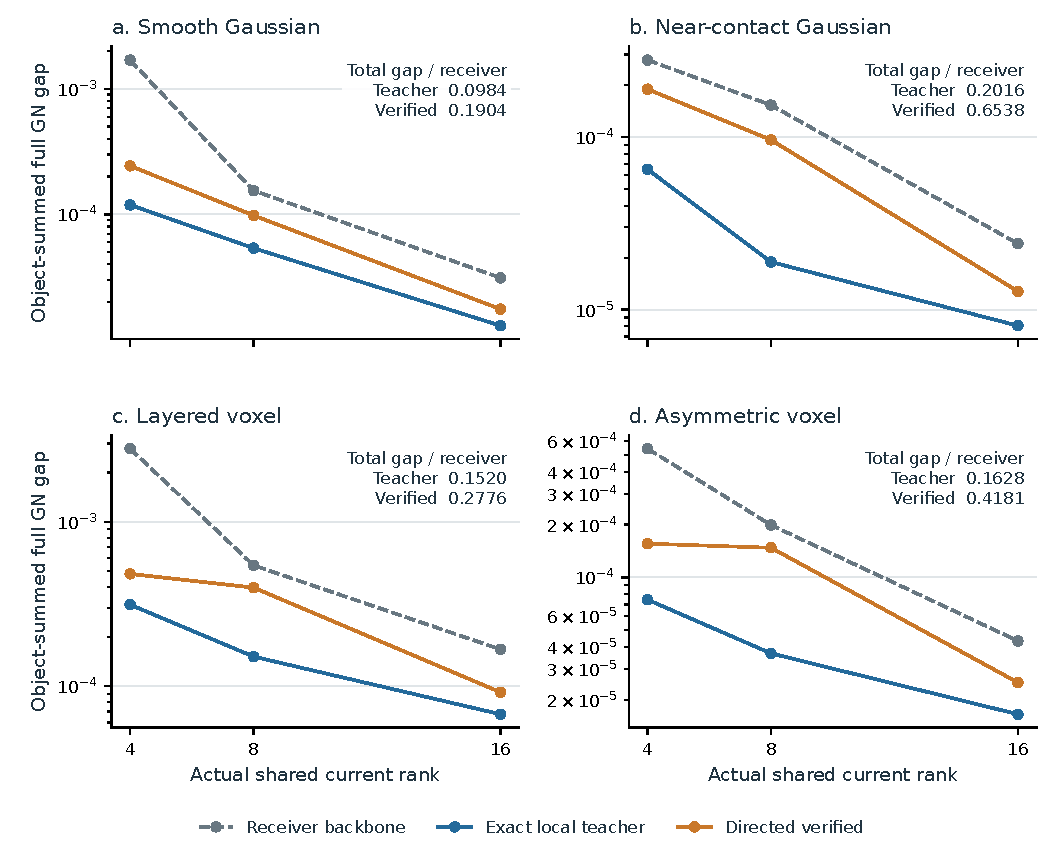
\includegraphics[width=.92\textwidth]{figures/exchange_risk.pdf}
\caption{Absolute complete-quadratic gaps summed over three states of each object at each current budget. The teacher exhausts a declared local exchange neighborhood; the verified method sees twelve incoming candidates and checks at most two finalists per round. The curves are descriptive object summaries, not 36 independent objects or nonlinear reconstruction errors.}
\end{figure*}

We separate proposal error from omitted opportunity at the common receiver checkpoint. With the full dictionary available, anchor top-one ranking captures 98.1--99.6\% of the object-summed best one-decision gain. The twelve-incoming pool contains 35.3\%, 91.98\%, 96.89\%, and 65.89\% of that opportunity for the near-contact, layered, smooth, and asymmetric objects. The near-contact result is therefore mainly a shortpool limitation at this checkpoint, rather than a large full-dictionary ranking error. This diagnosis does not equate differing multi-action paths with pure score regret.

The rank-at-most-$k$ policy ends at $k$ in every cell. It produces a different path in one case but demonstrates no terminal rank saving. Verified exchanges accept 75 actions, paying 1164 finalist tangent RHS in addition to the separately recorded initialization and screening costs. Twenty-two cells stop unresolved and fourteen reach their move budget. No complete-neighborhood stopping certificate is established.

\subsection{Information growth can accompany a worse step}
Information diagnostics cover a fixed twelve-incoming subset per removal, with the teacher-best move separately added when absent. Complete information spectra are available on the Gaussian material spaces; voxel metrics use the common sixteen-direction projection. The augmented diagnostic subset is utility-biased and is not a prevalence sample of all current directions.

For one resolved near-contact initial-state replacement at $k=4$, information volume increases by 6.3127 and effective dimension by 1.8613, while the actual complete-quadratic gain is $-5.5754\times10^{-5}$. The normalized curvature fidelity also improves slightly. Thus neither information magnitude nor this fidelity scalar determines the signed update utility. Equation~\eqref{eq:information-offset} identifies the missing residual-dependent term.

\begin{figure*}[tbp]\centering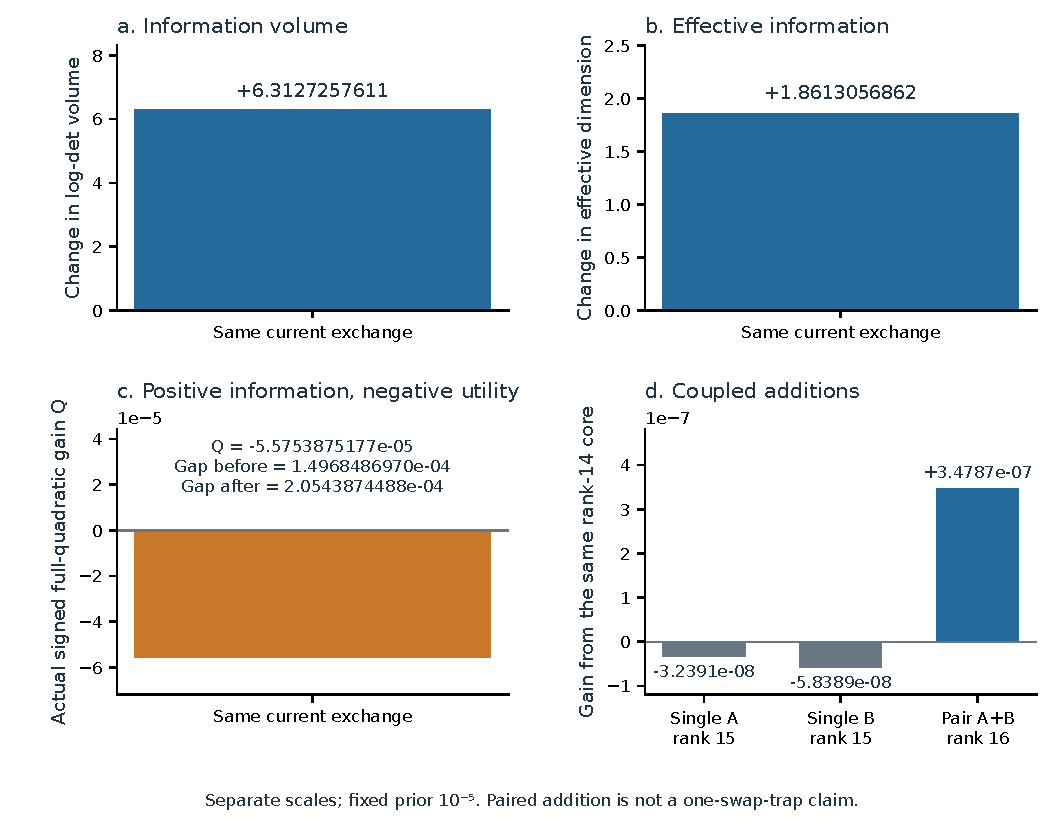
\includegraphics[width=.90\textwidth]{figures/information_and_pair_witness.pdf}
\caption{Left: a physical Maxwell replacement increases both information-volume and effective-dimension diagnostics but worsens the actual material step. Separate axes retain their different units. Right: from a common rank-14 core, two rank-15 singleton additions have negative gain, while their rank-16 joint addition has positive gain. This is an addition-interaction witness, not a same-rank 1-swap trap.}
\label{fig:information-pair}
\end{figure*}

Five strict joint-addition witnesses occur in the 540 fixed-core pair tests. One has singleton gains $-3.2391\times10^{-8}$ and $-5.8389\times10^{-8}$, but joint gain $3.4787\times10^{-7}$. Candidate coupling can therefore defeat independent singleton decisions. On a separate common-candidate diagnostic, mandatory top-one selection using linear evaluation of actual displacement chooses negative-gain endpoints in 29 of 36 cells; complete quadratic evaluation reduces this count to one. Scoring a linearized displacement and executing the actual endpoint also retains substantial mismatches. The deployed acceptance includes no-op and rejects negative gains. This controlled diagnostic replaces a causal interpretation of the older, confounded finite/first-order policy ratio.

\subsection{What the checks cost and what remains untested}
Two representative early states use the same CUDA FP64 endpoint and physical direction-action backend for five rotated timing repetitions. Median warm selection time for the conditional method is 0.594, 1.418, and 2.690~s on the near-contact Gaussian state at $k=4,8,16$, and 0.891, 1.153, and 3.400~s on the layered voxel state. One directed decision using the same initial shortpool costs 0.328--0.937~s and 0.333--1.215~s, respectively. The cached fixed-onepass control costs 0.113--0.219~s and has different proposal semantics. Conditional verification buys fidelity with additional screening and physical actions; these timings establish no acceleration over unchanged receiver selection. Historical cache acquisition is separately recorded, while independent cold speedup remains unmeasured.

A fixed two-architecture, three-seed CPU priority pilot uses object-grouped train/validation/test partitions. On the single heldout asymmetric object, MLP top-two opportunity capture is 98.85--99.16\%; group-mean capture is 75.99--98.03\%. Every run is below anchor top-two capture, 99.885\%. These labels evaluate offline priority, with no new physical acceptance test or measured all-in feature-cost saving. Learned proposal is therefore not retained as an algorithmic contribution.

The full-reference Gaussian direction decomposition reproduces archived risk changes to relative error below $6.5\times10^{-11}$. All six Gaussian states have zero full-reference weak directions under the declared threshold $\nu\le1$ and scale $P=10^{-5}I$. Weak directions suggested by a reduced model cannot be treated as verified full-material prior freedom. The voxel projection cannot resolve weakness in the entire material space.

Finally, the unconstrained unit-step truth diagnostic improves material error relative to the current state in 19 cells and worsens it in 17; 28 steps violate the material constraints. No nonlinear exchange reconstruction is run. The evidence supports conditional frozen-update design, with output-error certification, economical proposal construction, noise, and accepted nonlinear transfer remaining open.
